\chapter{Introduction}

\section{Motivation: we subtract for space and for sound, almost never for sight}

We already delete distraction, and we have done it for a long time, but only in two of the three
senses that matter for concentrated work.

For \textbf{space}, the instrument is the library carrel. Wooden walls on three sides. Nothing is
added to help anybody read. The room is simply taken away until only the page is left, and the design
has survived for centuries because it works.

For \textbf{sound}, the instrument is the noise-cancelling headphone. It does not make the audio
louder. It just makes all the other sounds quieter. It is a product people buy, at a reasonable
price. And its entire function is removal, with an architecture of a microphone, a processing stage
and a speaker.

For \textbf{sight} we have nothing comparable today. What we do have is a description of the
\textit{state of mind} such an instrument would produce, and it is the oldest description of it we
have, in the
Mah\=abh\=arata\footnote{The Mah\=abh\=arata is an ancient Sanskrit epic of India. The archery
lesson retold here is one of its best-known episodes.}. Dro\d{n}a, the martial teacher of the P\=a\d{n}\d{d}ava and Kaurava princes, sets up
a wooden bird in a tree and tells his students to aim for its eye. Before each releases the arrow, he
asks what they see. One says the tree. Another the branches and the leaves. Then Dro\d{n}a turns to
Arjuna and puts the question to him one thing at a time. Do you see the tree? No. The branches? No.
Your brothers standing beside you? No. ``I see only the eye of the bird.'' For that moment the tree,
the branches, and everyone else standing there have not merely fallen out of Arjuna's interest. They
have gone.

That is three thousand years of treating removal as the definition of visual focus, and the tools we
actually build for vision do the opposite. Every visual attention aid in common use adds something
to the scene. This dissertation asks what the missing instrument looks like: the carrel and the
headphone, applied to sight, on hardware people already own.

The need is not hypothetical. The modern visual environment is engineered against sustained
attention. Open-plan offices place moving colleagues at the edge of vision. Shared homes put
televisions and phone screens beside
workspaces. Streetscapes compete for a driver's gaze with advertising designed by professionals to
win it. The cost is well documented: task-irrelevant peripheral events capture attention
involuntarily, and each capture carries a performance penalty on the task the viewer intended to do.
In immersive settings the effect is directly measurable. Introducing peripheral visual distractors
into a virtual classroom more than doubled commission errors, responses to stimuli that should have
been ignored, on a sustained-attention task in a recent study of sixty-six participants
\citep{ai2025}, replicating decades of laboratory findings on involuntary attentional capture by
peripheral motion and luminance change \citep{itti1998}.

The extended-reality (XR) community's response has been additive in exactly the way the carrel and
the headphone are not: arrows, halos, attention funnels and highlights layered onto the world to
point at what matters \citep{biocca2006}. This dissertation pursues the complementary and far less
explored operation, \textit{subtraction}. If the periphery pulls attention away, dim it, mute it, or
re-grade it so that it pulls less. In the literature this family of operations is called diminished
reality (DR), concealing or attenuating real-world content rather than adding to it
\citep{mori2017,cheng2022}, and its application to distraction has recently been named \textit{visual
noise cancellation}, by direct analogy with the acoustic kind \citep{hong2024}. The analogy is also
architectural: a headset's camera, processing stage and display mirror a headphone's microphone,
processing stage and speaker (Figure~\ref{fig:anc}).

\begin{figure}[htbp]
\centering
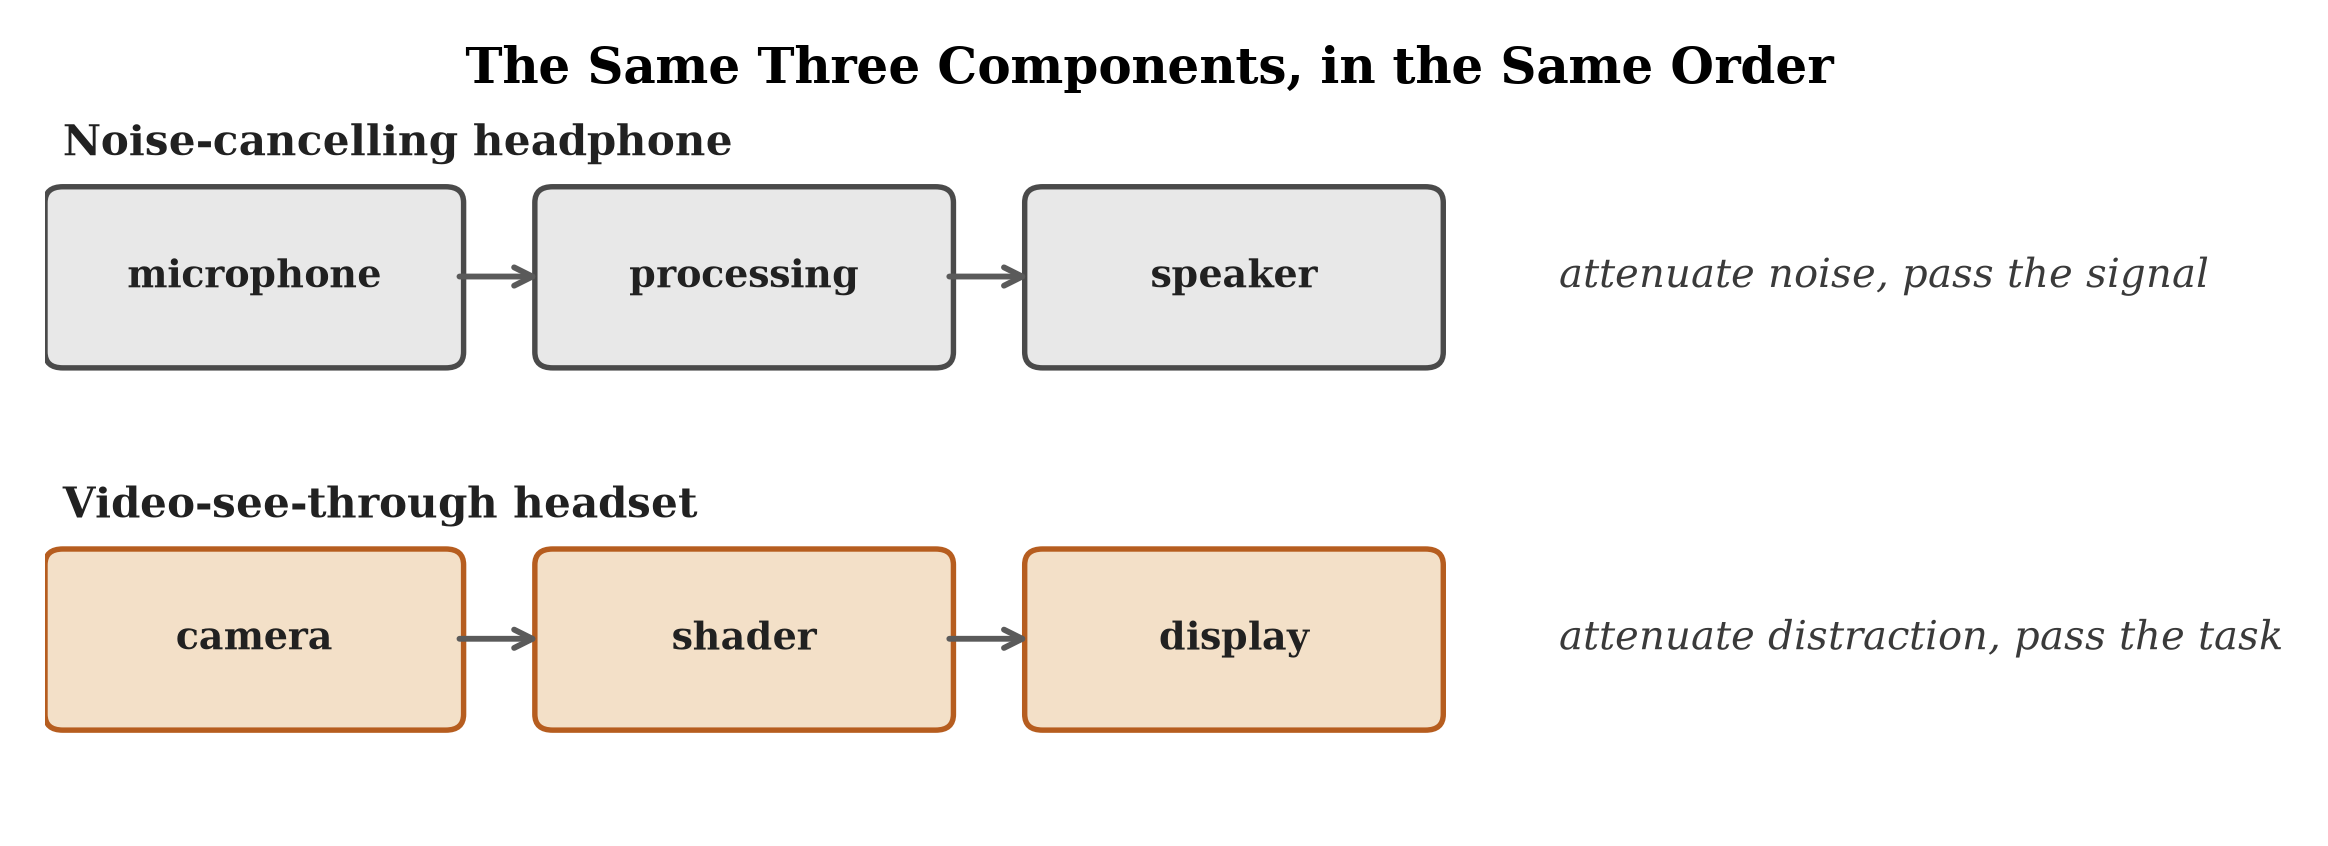
\includegraphics[width=\linewidth]{content/figures/fig_anc_analogy.png}
\caption{The noise-cancellation analogy as architecture: capture, process, re-present. The
headphone attenuates noise and passes the signal; the headset attenuates distraction and passes the
task.}
\label{fig:anc}
\end{figure}

A video-see-through (VST) headset is, in principle, the ideal instrument for visual noise
cancellation. Unlike optical see-through glasses, whose additive light engines physically cannot
darken the world, a VST headset re-displays the world on an opaque screen, so every pixel the user
sees is in principle available for modification. The Meta Quest 3, an affordable and widely owned
consumer device with colour passthrough, would seem to make DR-based attention guidance deployable at
scale for the first time. In principle.

\section{The compositing constraint}

In practice the premise that every pixel is available for modification is false on consumer hardware,
and that falsity is the motivating technical problem of this dissertation.

On the Quest 3 the passthrough view of the world is composited by the operating system, not by the
application. An application cannot read the passthrough layer, cannot shade it, and cannot spatially
mask it. It may only draw \textit{on top} of it, or apply a global colour transform through a narrow
styling interface. Since early 2025 the platform has additionally exposed the raw forward camera feed
to applications through Passthrough Camera Access, but at materially lower quality than the system
passthrough the user normally sees: a monocular 1280$\times$960 stream covering roughly
85--90$^{\circ}$ of field of view, against the system layer's full coverage of the headset's
approximately 110$^{\circ}$ display with its correct per-eye reprojection. The one place where full
pixel control exists is therefore also the place where image quality is worst. A recent
psychophysical study shows the stakes plainly: no current VST headset reaches normal human visual
acuity through its passthrough, and the Quest 3 degrades further in low light \citep{wang2026}.

Subtractive attention guidance on this platform therefore poses a \textit{compositing-rights}
problem. The effect one wants, dim everything except the region that matters without degrading the
region that matters, cannot be obtained by editing the image the user sees, because no application is
permitted to edit it. Chapter 3 shows that what remains is a narrow but genuinely usable design
space, organised into three tiers of access, and Chapter 4 presents a working system exploiting an
architectural inversion at its centre. The region that matters is rendered as an \textit{absence}, a
transparent window in an overlay, so that the highest-quality image on the device, the native system
passthrough, serves the focus region for free, while the manipulation is confined to the periphery
where acuity is lower and precision matters less.

A mode is one named recipe for manipulating the periphery, and
the system implements ten of them. Three matter for this dissertation. \textbf{Hard Dark} blacks the
periphery out completely. \textbf{Soft Dark} dims it partially, leaving events visible through the
veil. \textbf{SignPop} re-grades a camera copy of the periphery towards dim grey, sparing signal
colours, and lifts a confirmed signal lamp or sign to full visibility. Figure~\ref{fig:treatments} shows the
two evaluated modes, Hard Dark and SignPop, alongside Soft Dark, as the user sees them. The most
capable of these configurations composites native passthrough inside the window with a
shader-processed camera feed outside it, a hybrid for which a structured prior-art search found no
published or shipped precedent.

\begin{figure}[htbp]
\centering
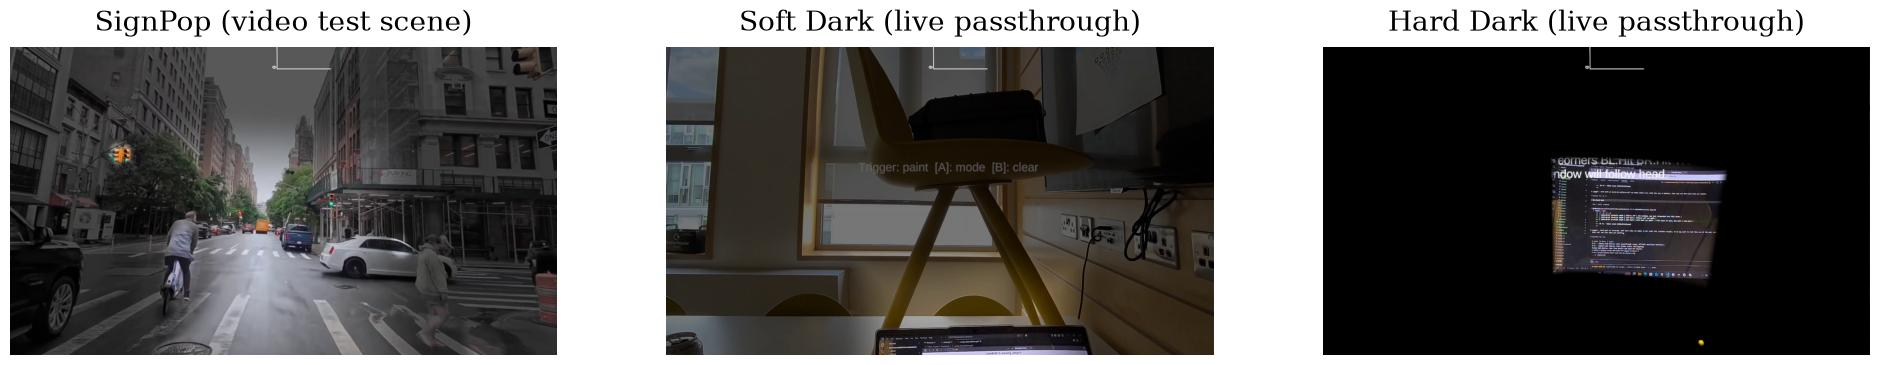
\includegraphics[width=\linewidth]{content/figures/fig_treatments.jpg}
\caption{The two evaluated treatments and Soft Dark, seen from the user's viewpoint, from on-device
recordings.
SignPop is shown in the video test scene it is evaluated in; Soft Dark and Hard Dark are shown over
live passthrough of a real room, each with the world-locked focus window revealing untouched
passthrough.}
\label{fig:treatments}
\end{figure}

\section{One question, two halves}

The dissertation asks a single question, with two distinct halves:

\begin{quote}
\textbf{Can subtractive attention guidance be delivered on consumer XR hardware? And when it is
delivered, does it actually help people focus?}
\end{quote}

\textbf{Part T (technical): can it be built?} What degree of diminishment control is achievable on a
consumer VST headset without OS-level access to the passthrough layer, and at what cost to image
quality, field of view, latency and comfort? Part T is answered by the design space of Chapter 3 and
the reference implementation of Chapter 4.

\textbf{Part H (human): does it work?} Under controlled distraction, does peripheral diminishment
reduce the cost distractors impose on a focal task, and does salience re-grading enhance focal
detection without unacceptably degrading peripheral awareness? Part H is answered by the
pre-registered user study of Chapter 5.

Two methodological commitments connect the halves and should be named at the outset, because they are
choices rather than accidents. First, the study's dynamic scenario runs as a \textit{simulation},
pre-recorded driving footage presented on the system's rendering sphere rather than live passthrough
of a street, following the closest published DR evaluations, which simulated diminishment inside
virtual environments because controlled, repeatable, event-dense stimuli cannot be obtained from the
uninstrumented real world \citep{cheng2022,mclaughlin2025}. Second, detection is supplied by an
\textit{oracle} computed offline over the study footage rather than by a model running on the
headset, so the study can ask whether an effect built on excellent detection helps attention without
first engineering excellent detection on-device.

The two study blocks bracket the feasibility spectrum. The primary, workstation, block runs on
\textit{real passthrough with real physical distractors}, the actual artefact with no simulation. The
secondary, driving, block evaluates the concept in the simulated deployment context.

\section{Research questions and hypotheses}

The dissertation's question breaks into three research questions. Each confirmatory research
question is answered by one or more pre-registered hypotheses, a specific, testable prediction with
a named condition and measure. \textit{Pre-registered} here means the hypotheses, margins, tests and
decision table were frozen and lodged with the supervisor in a written memo before data collection
began (Appendix A, Sections A.3 and A.6). No external registry was used, and the claim made throughout is that
these choices predate the data, not that a third party holds them. RQ1 carries the single primary
hypothesis (H1). RQ2 carries two
secondary hypotheses, a benefit prediction (H2a) and a safety prediction (H2b). RQ3 is exploratory
and carries no hypothesis. The full pre-registered forms, including smallest effect sizes of
interest, equivalence margins, statistical tests, and a decision table committing the dissertation
to a conclusion under every outcome, are given in Chapter 5.

\begin{itemize}
\item \textbf{RQ1 (primary).} Does dimming the periphery reduce the performance cost that peripheral
  visual distractors impose on a focal task? The study tests this with the Hard Dark mode and a
  world-locked focus window, on a workstation task.
\item \textbf{RQ2 (secondary).} Can salience re-grading improve detection of relevant peripheral
  events without degrading detection overall? The study tests this with SignPop on a driving scene:
  a benefit prediction where the re-grading has room to act, and a safety prediction that detection
  pooled across the whole scene stays within an acceptable margin of the untreated view. The safety
  prediction is tested by equivalence, so a failure to establish it would carry more information than
  an ambiguous null. As it turned out, the two-sided statistic was not established, for a
  one-directional reason that Chapter 5, Section 5.7.2 and Chapter 6 report as a specification
  mismatch rather than a safety result.
\item \textbf{RQ3 (exploratory).} After experiencing the system, what do participants report about
  perceived focus benefit, perceived awareness cost, and visual comfort?
\end{itemize}

The study is built so that every outcome maps to a pre-committed conclusion. Distractors are already known to impose
a measurable cost \citep[N = 66]{ai2025}. The study takes that cost as given, asks whether the
system reduces it, and pre-commits to the interpretation of every outcome, including failure.

\section{Contributions}

\begin{itemize}
\item \textbf{C1: Design space.} A taxonomy of what DR is and is not achievable under the
  compositing constraints of consumer VST hardware, with the ceilings and costs of each kind of
  access, characterised from implementation experience rather than speculation (Chapter 3).
\item \textbf{C2: Reference implementation.} An open, working multi-mode DR attention-guidance
  system on Quest 3 passthrough. Its main technical elements are a world-locked focus window
  rendered as an absence in the overlay, a world-direction sampling scheme that lets the monocular
  camera feed fuse binocularly, motion-coupled comfort suppression, and ten peripheral treatments
  spanning the design space of Chapter 3. Two of them, SignPop and Hard Dark, are carried to
  confirmatory evaluation, with documented failure cases and with the architecture's two central
  trade-offs, frame cost and legibility, measured on device (Chapter 4). The full source code is
  publicly available at \url{https://github.com/batunii/Arjuna}.
\item \textbf{C3: Pre-registered user study, carried to analysis.} A within-subjects study designed
  so that any outcome is informative: one primary hypothesis powered close to its design target, a
safety check with
  a pre-set margin on how much peripheral awareness may be lost, pilot checks that gate the design,
  and a decision table committing the dissertation to a conclusion under every outcome. It is
  reported with the full analysis of the nineteen workstation and seventeen driving pairs collected,
  read against that table (Chapter 5).
\end{itemize}

\section{Scope: what this dissertation does not claim}

Because the credibility of a small, carefully scoped study depends on the discipline of its claims,
the non-claims are stated as prominently as the claims.

\textbf{No driving or road-safety claims.} The driving footage used in the secondary study block is a
dynamic, high-event-rate monitoring \textit{stimulus}. A seated participant passively watching
passenger-perspective video licenses no inference about driving, drivers, or road safety. Such
inference would require a driving simulator with vehicle control, which is out of scope.

\textbf{No product claims.} The study evaluates attention mechanisms under controlled distraction,
not the desirability or readiness of a wearable product. Comfort findings from a 2026 headset
transfer to future lighter hardware only as bounds, and are reported as such.

\textbf{Oracle conditioning stays visible.} SignPop's finding depends on detection, and specifically
on offline oracle-quality detection rather than live on-device detection. The gap between the two was
never measured, so every place this dissertation reasons about a deployed detector-driven system,
that reasoning is conditioned on the oracle assumption and marked accordingly. Oracle performance is
never substituted for live performance without saying so.

\textbf{Two technical measurements, not a benchmark campaign.} Chapter 4, Section 4.11 reports two
on-device measurements: per-mode GPU frame cost against the display budget, and legibility of the
native passthrough path against the camera re-render. No latency, world-locking stability, or
thermal-endurance measurement was performed, so where those properties are argued, they are argued
from the structure of the system rather than from a measured number.

\textbf{Analysed sets smaller than the tested sample.} The pre-registered twenty
participants completed the full two-block protocol. The workstation block
lost one pair, P1's, whose arm assignment could not be verified from the session ledger, and the
driving block lost three pairs to its response-validity and comprehension exclusions. The
final counts are nineteen usable pairs for the workstation block and seventeen for the driving block,
at 79.8\% and 89.0\% achieved power (two-tailed) for the primary contrast and the pre-registered
eccentricity band.
The pre-committed decision table is applied to this sample, and where a verdict is weaker than the
headline number suggests, the weaker verdict is the one reported.

\textbf{Mode-in-context claims, not mode-generalised ones.} Each mode was tested in one scenario:
Hard Dark in the workstation block, SignPop in the driving block. Mode and scenario are therefore
confounded by design, and nothing in the study separates them. Every confirmatory claim is a claim
about a mode in its context, never about the mode in general.

\textbf{No attribution to any single effect.} A SignPop detection fires a bundle of six visual
changes at once, so the 20--30$^{\circ}$ benefit is attributed to the bundle and not to any one of
its components (Chapter 4, Section 4.5.5).

\textbf{Soft Dark carries no participant data.} Of the three modes that matter for this
dissertation, only Hard Dark and SignPop were placed in front of a participant. Soft Dark is
design-space material throughout, and no empirical claim is made about it.

\begin{figure}[htbp]
\centering
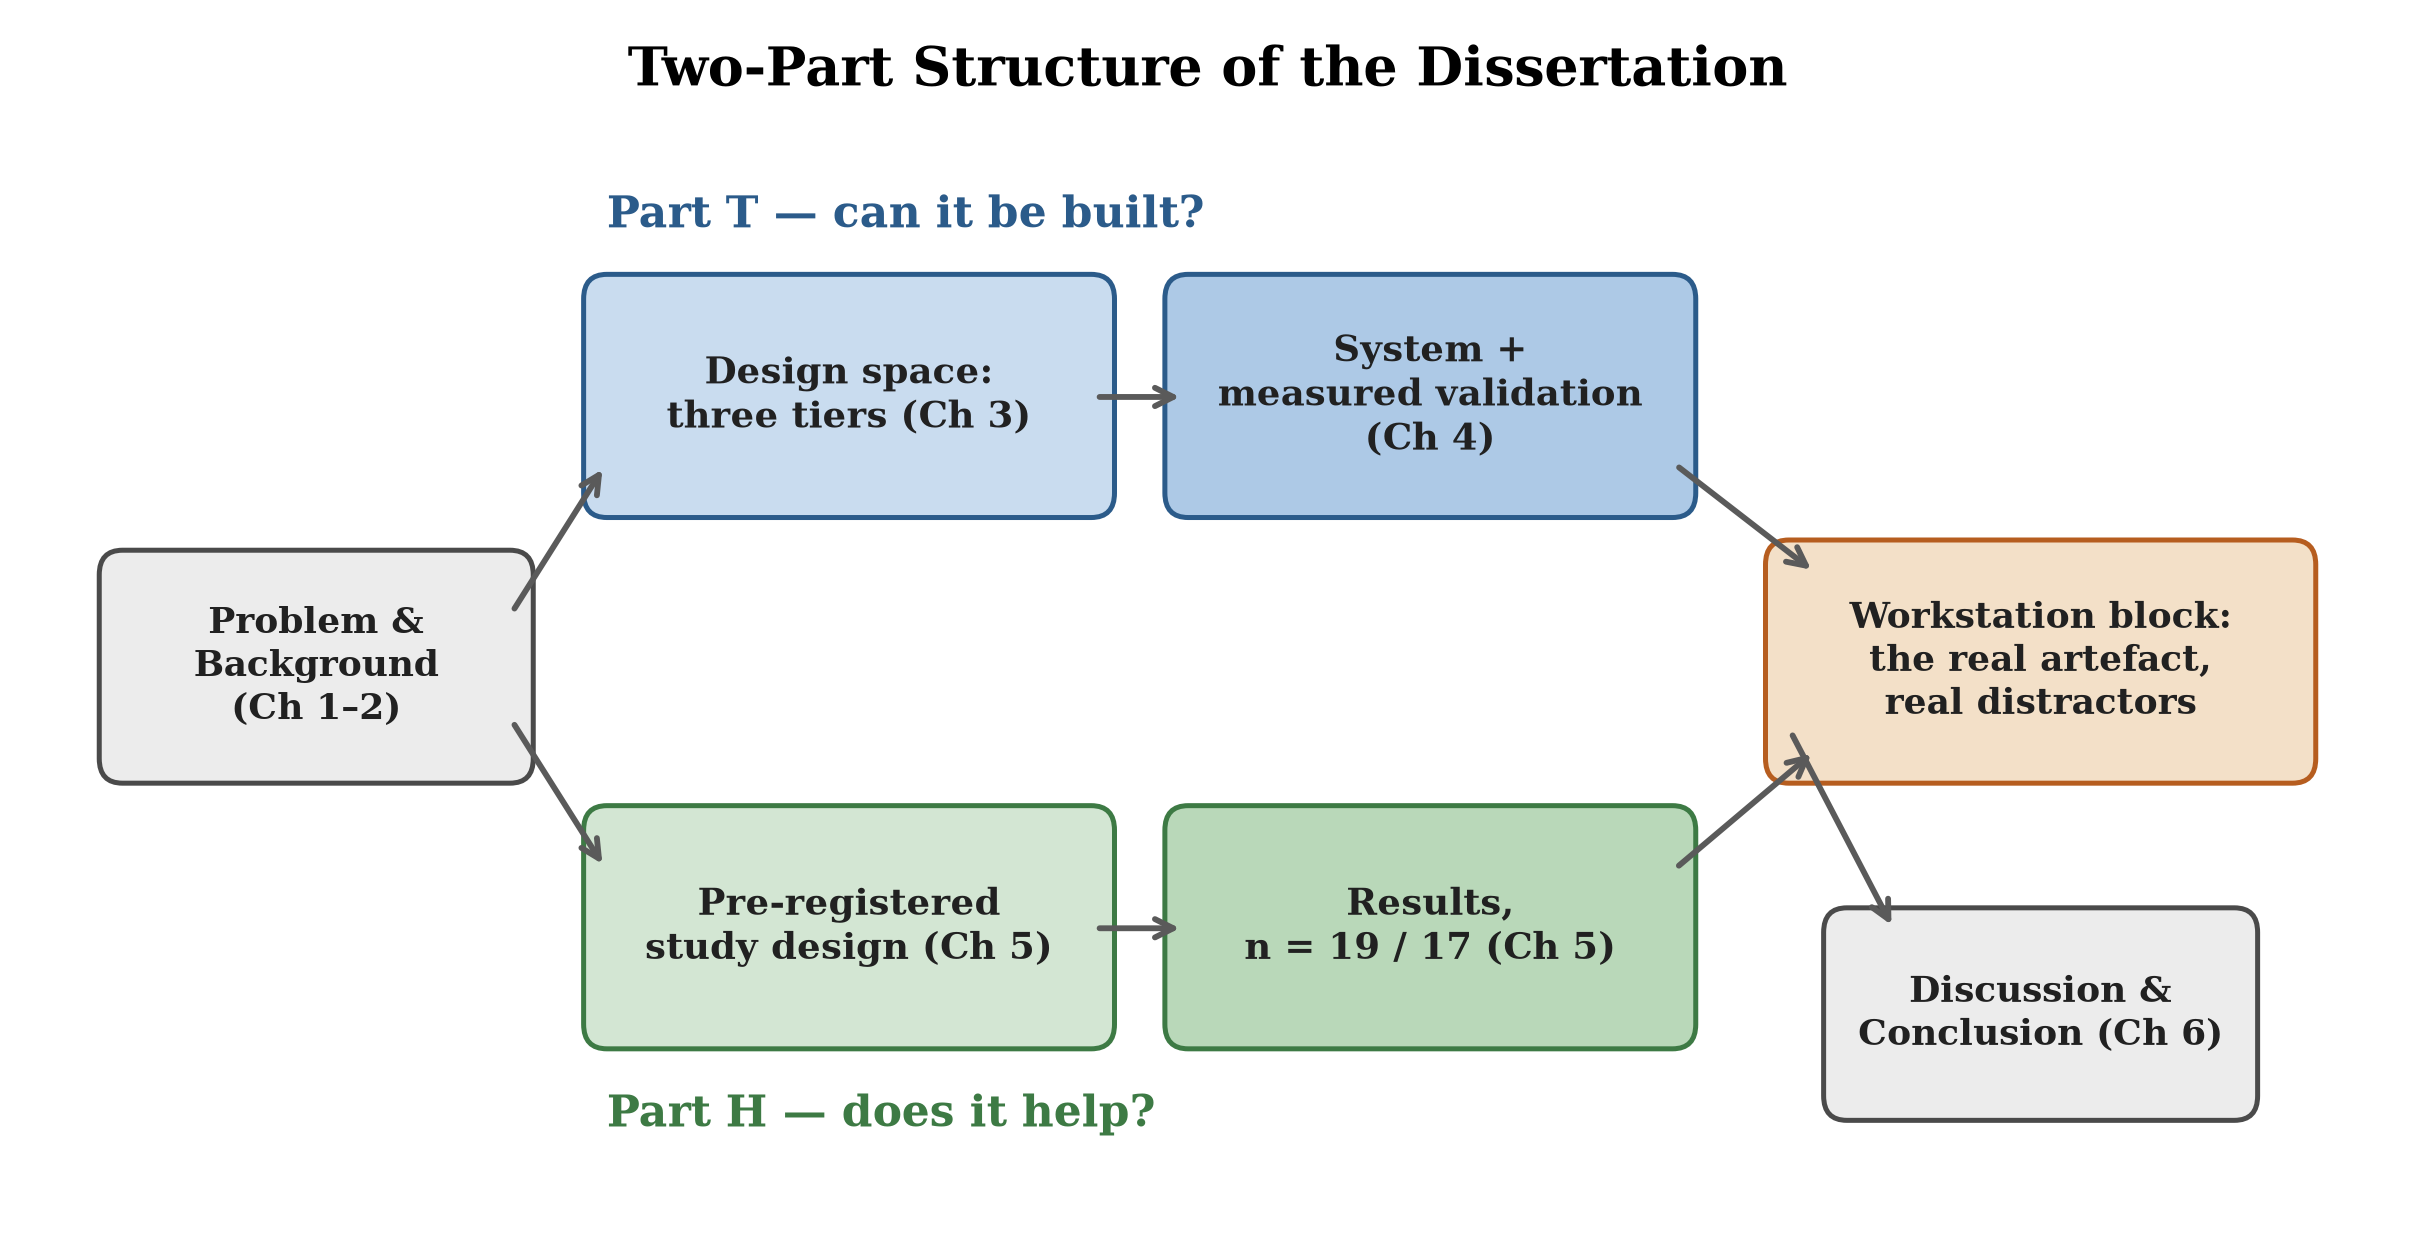
\includegraphics[width=\linewidth]{content/figures/fig_dissertation_structure.png}
\caption{The two-part structure of the dissertation.}
\label{fig:structure}
\end{figure}

Figure~\ref{fig:structure} sets out how the two parts of the dissertation fit together, with the
workstation block bridging them on real hardware.
